During the development of the Data Discovery Library, it was suggested that it would be
nice to have a visual way of communicating the results of the library,
and the general structure of the analysed files.

As a solution, a simple tool was created which can take a list of metadata, and
generated a graphviz file.

\begin{figure}[H]
    \centering
    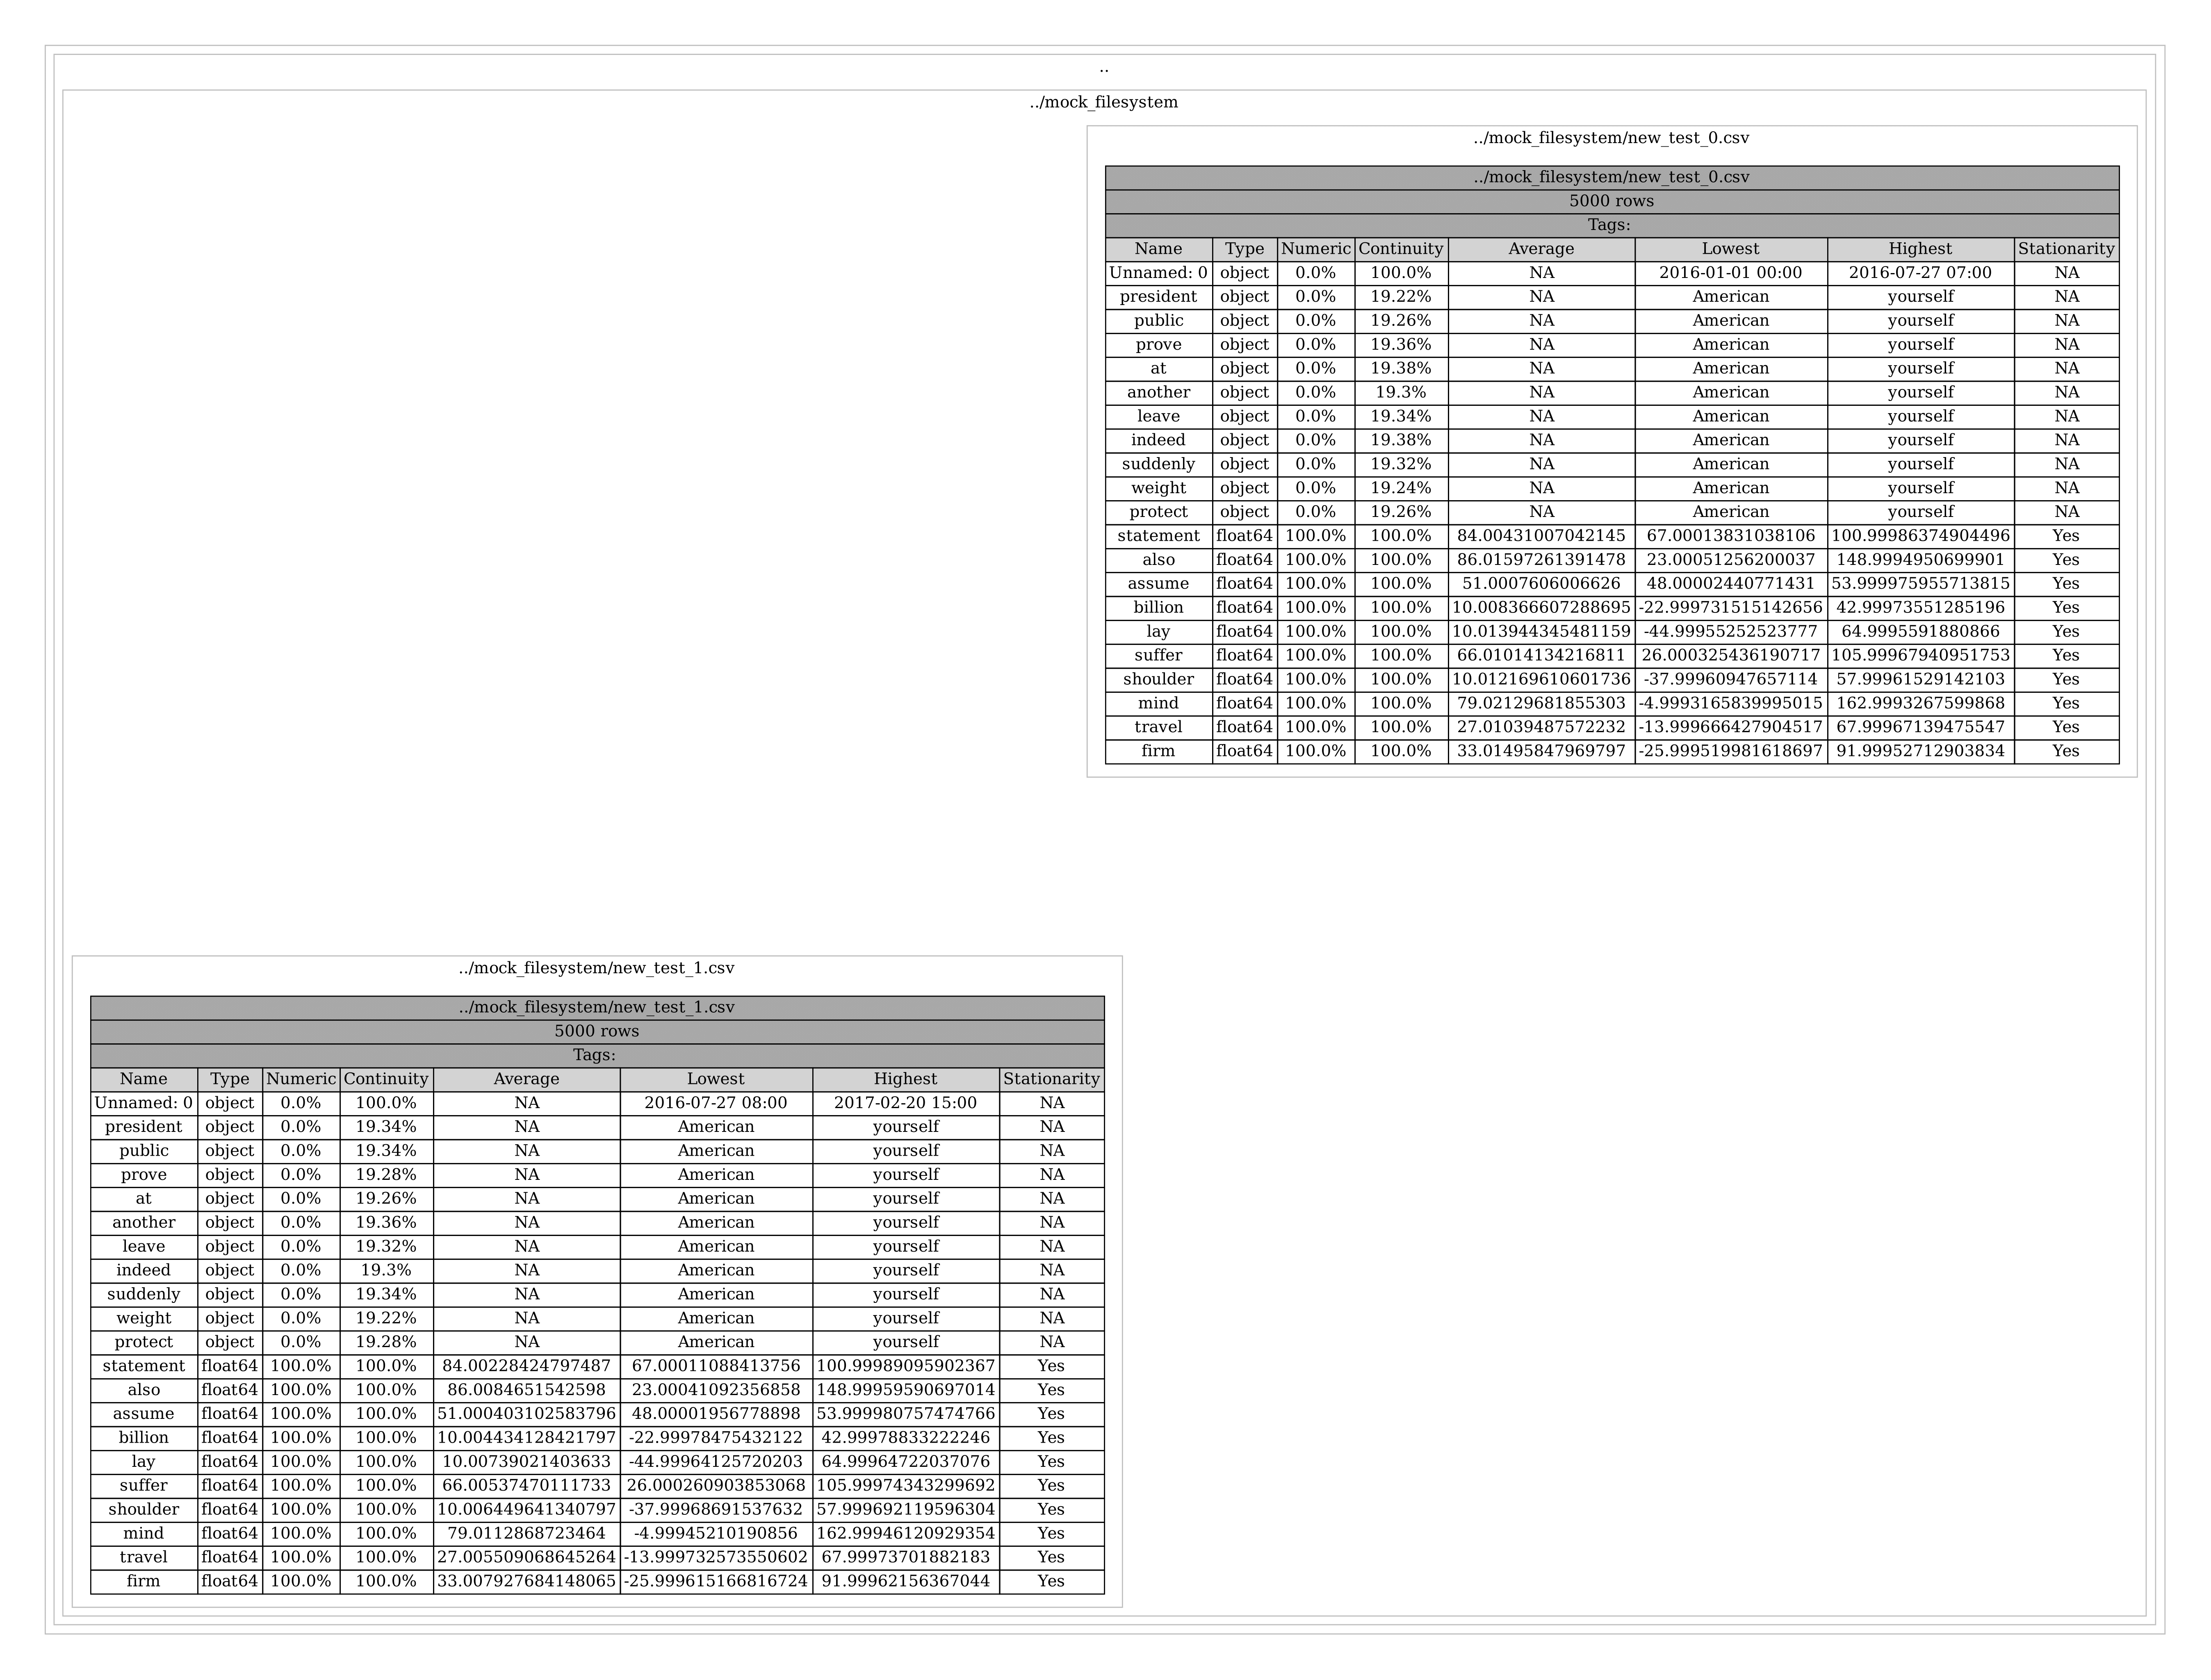
\includegraphics[width=12cm]{figures/metadata_visualization/visualized-1}
    \caption{Rendered output of the metadata visualizer}
    \label{fig:metadata_vis_fig_1}
\end{figure}


An example output is shown on ~\ref{fig:metadata_vis_fig_1}.
Graphviz, as the backing format was chosen because it had a relatively simple,
human-readable syntax - in some cases it even uses HTML tags, for example for tables.
Ultimately, it did become too limiting, when attempts were made
to implement things like relationships across columns.

Internally, to generate the correct structure, the visualizer tries
to build a tree based on the metadata filepaths.

Since the metadata are not guaranteed to be ordered based on depth, the visualizer
iterates through all of them first, ensuring that all possible levels have been addressed
(based on the file paths) and only then renders the graph.


